\documentclass[../main.tex]{subfiles}
\begin{document}
\section{Results}
\subsection{$2 \times 2$ lattice, analytical expressoins}
If we scale the value of $\beta$ from $1/k_BT$ to $1/J$ (Scaling factor $k_B T/J$) in the analytical expression from section \ref{sec:theory-analy}, we will get a good benchmark for computer computations to come. These values are listed in table \ref{tab:2x2spinsEnergiesMags} below. Note that all values are divided by four, since we want the values per bond, and not for the entire lattice.
\begin{table}[!h]
\begin{center}
  \begin{tabular}{l r}
    Mean energy, $\langle E \rangle$: & $-1.9960$  \\
    Mean absolute magnetization, $\langle |\mathcal{M}| \rangle$: & $0.9987$ \\
    Specific heat capacity, $C_V$: & $0.0321$\\
    Susceptibility, $\chi$: & $3.9933$
  \end{tabular}
  \caption{Benchmark for material characteristics per bond for a $2 \times 2$ lattice}
  \label{tab:2x2spinsEnergiesMags}
\end{center}
\end{table}
\FloatBarrier

\subsection{Ising model: simulation over temperature}
We ran the program for different amounts of Monte Carlo cycles and plottet the error (analytical - simulated) in figure \ref{fig:results-MCplot} below. It seems we want to use around $10^{7}$ MC cycles or more to get a good simulation.

\begin{figure}[!h]
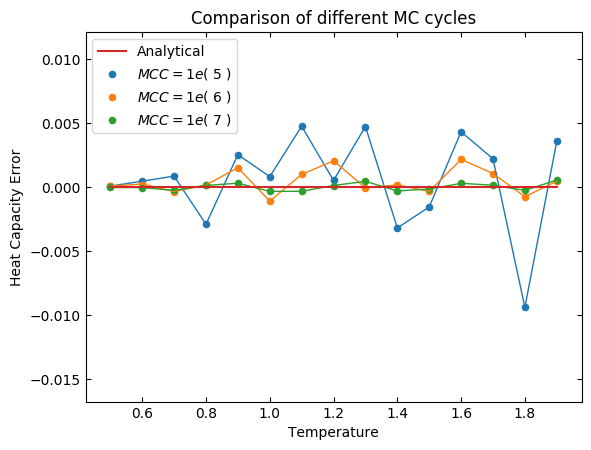
\includegraphics[scale=0.7]{CyclesComparison.png}
\caption{Shows the accuracy of different amount of MC cycles over temperature.}
\label{fig:results-MCplot}
\end{figure}
\FloatBarrier


\end{document}
